\begin{figure*}
\centering
\begin{multicols}{3}
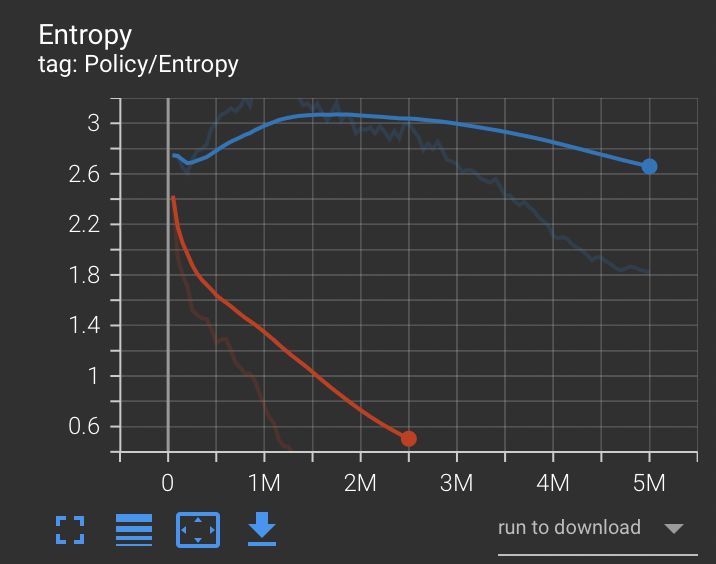
\includegraphics[width=0.99\columnwidth]{Chapter3/beta/beta_entropy.png}\par
\caption{Lower beta of 0.001(red) able to achieve lower entropy than higher beta of 0.01(blue) }
\label{fig:beta_entropy}

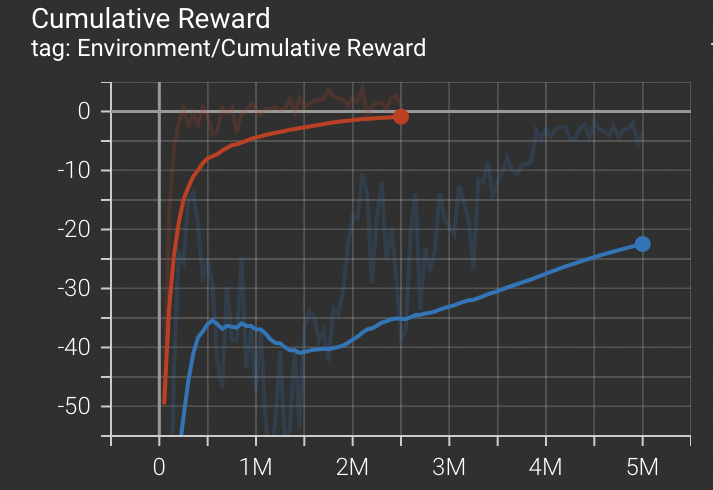
\includegraphics[width=0.99\linewidth]{Chapter3/beta/beta_cumu_reward.png}\par
\caption{Lower beta of 0.001(red) able to achieve higher cumulative external rewards than higher beta of 0.01(blue).}
\label{fig:beta_cumreward}

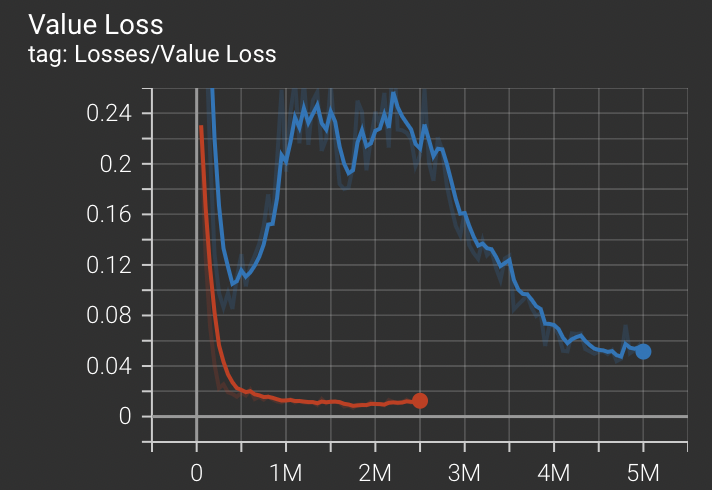
\includegraphics[width=0.99\columnwidth]{Chapter3/beta/beta_value_loss.png}\par
\caption{
Lower beta of 0.001(red) able to achieve lower policy loss than higher beta of 0.01(blue) 
}
\label{fig:beta_valueLoss}
\end{multicols}
\end{figure*}
